%!TEX root = Abschluss-ML-Prak-2015.tex
%SEBASTIAN
\section{Ergebnisse}

\subsection{Ergebnisse}

\begin{frame}{Ergebnisse-Convolutional Layer}
 
    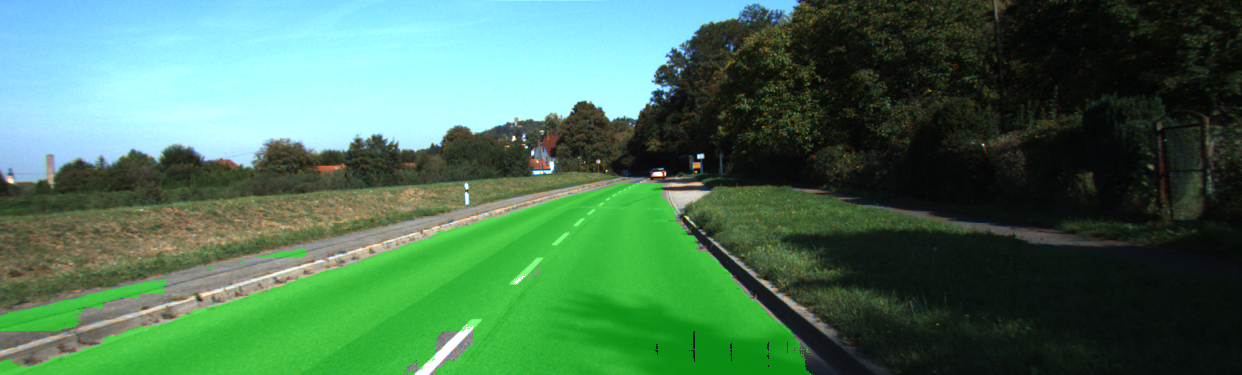
\includegraphics[scale=0.2]{../images/Convolutional/um_000014+-overlay-fully-49-patch.png}
\end{frame}    
    
 \begin{frame}{Ergebnisse-Convolutional Layer}
 
    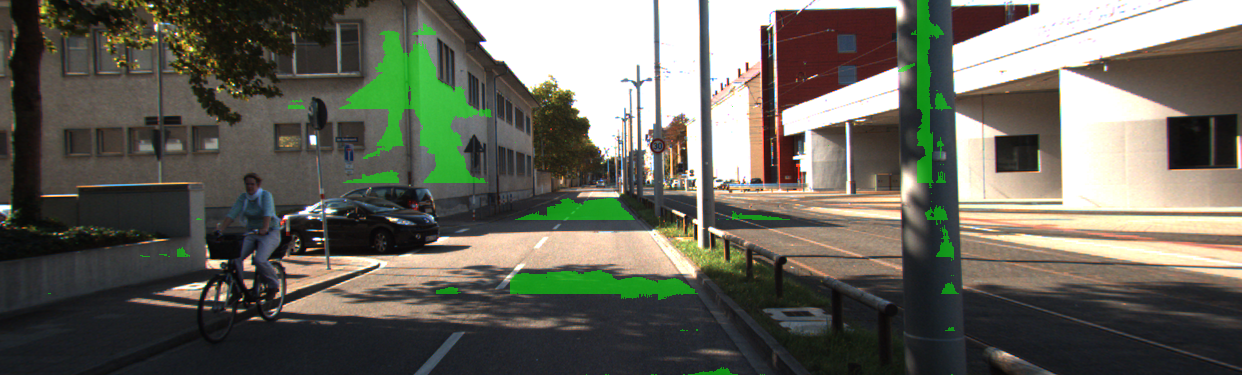
\includegraphics[scale=0.2]{../images/Convolutional/um_000066-overlay-fully-49-patch.png}
 \end{frame}     

\begin{frame}{Vergleich}

      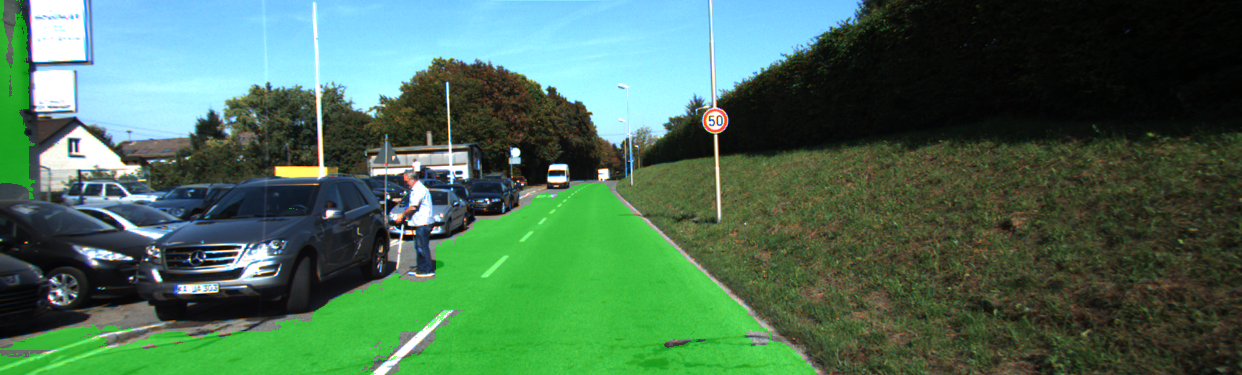
\includegraphics[scale=0.2]{../images/Convolutional/um_000014-overlay-fully-49-patch.png}
         \vspace{0.1cm}
    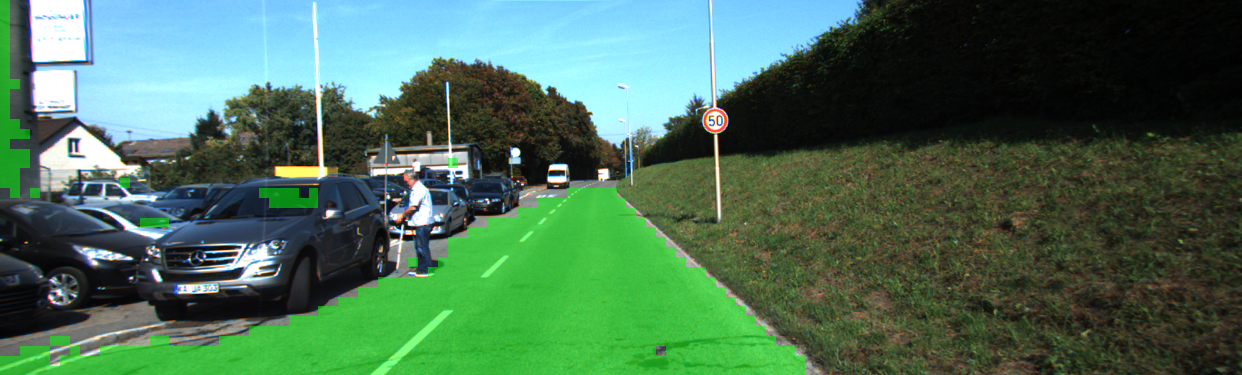
\includegraphics[scale=0.2]{../images/Convolutional/um_000014-overlay.png}

\end{frame}

\begin{frame}{Vergleich}

      False Positive Negative .....

\end{frame}

\begin{frame}{Laufzeiten}

      False Positive Negative .....

\end{frame}

\begin{frame}{Video}

      Video

\end{frame}

\section{Ausblick}
\subsection{Ausblick}
\begin{frame}{Ausblick}
    \begin{itemize}
        \item wegen zu wenig ram keine groesseren Patches
        \item Neuronales Netz verbessern
        \item effizienteres Zusammensetzten der Patches
    \end{itemize}

\end{frame}